In this chapter we discuss the experimental evaluation of DyPyBench. We do so by answering the following questions:

\textbf{RQ1:} How do the included test suites in Python projects within DyPyBench contribute to a dynamic benchmark?

\textbf{RQ2:} How efficient is our benchmark to generate (valid and good) training data for the neural models?

\textbf{RQ3:} How effective is DyPyBench to aid a comparison of static and dynamic call graph analysis?
Before answering the above questions, we detail the experimental setup for DyPyBench, neural model training and the call graph generation using static and dynamic analysis frameworks.
We further explain the evaluation criteria for measuring the effectiveness of DyPyBench.
% for the neural model and the analysis frameworks.
Finally, we discuss the evaluation and the results.

DyPyBench consists of 50 open-source python projects from different application domains list in Table \ref{table:50_installed_projects}.
We download the source code of these projects along with their test suite into a Docker image which contains the neural model (LExecutor) and the static (PyCG) and dynamic (DynaPyt) analysis frameworks.
We use these integrated test suites to execute the projects and collect various statistics and data.

\section{Experimental Setup for LExecutor}
We use DyPyBench to generate the training data for the neural model LExecutor.
LExecutor instruments the files and then generates traces from these files during run-time.
LExecutor provides its own instrumenter, and the accepts mandatory two arguments to perform instrumentation.
The first is a JSON file to store the mapping of iids and the second is files to instrument.
To generate the trace files, we execute the test suite consisting of the instrumented files.
The trace files from the above step are used to generate training data in the form of .pt files for the neural model.
For this task, LExecutor provides a module PrepareData which accepts the trace files and the JSON file created in the instrumentation step.
To generate the .pt file, LExecutor works in two modes of abstraction, fine-grained and coarse-grained.
At a time only one mode runs and this can be set in the Hyperparameters.py file.
The Listing \ref{code:Hyperparameters.py} shows the possible entries for the abstraction mode.
In this work, we generate the data using the two abstraction modes shown on line 1 and line 2 in the Listing \ref{code:Hyperparameters.py}. 
The PrepareData module also generates a validation file in the .pt format.
The trace entries are split into training and validation data based on the split provided in the Hyperparameters.py file as shown in Listing \ref{code:Hyperparameters.py} on line 3.
\begin{lstlisting}[caption=Abstraction Modes in LExecutor,label=code:Hyperparameters.py,language=Python]
    value_abstraction = "fine-grained"
    value_abstraction = "coarse-grained-deterministic"
    perc_train = 0.95
\end{lstlisting}

\section{Experimental Setup for PyCG}
PyCG generates call graph based on static analysis of code.
The call graphs is created in the JSON format, where the key is caller and the value is a list of called functions.
PyCG accepts 3 arguments, the package contains the source files, the entry point files and the output file save the JSON.
In DyPyBench, we provide the package as source code cloned from Git and the test files as entry point files for each project.
The execution of the PyCG module then provides us with the call graph in the mentioned JSON format.

\section{Experimental Setup for DynaPyt}
DynaPyt instruments the files and the execution of the instrumented code provides us with the dynamic analysis.
DynaPyt, has its own modules for instrumentation and analysis.
We first use the instrumentation module to instrument the source files.
To run the analysis, we create a entry file to run all the test files using the main function provided by the pytest module.
Additionally, we provide the option of import-mode set to importlib to the pytest.main function.
We add the Call Graph analysis is DynaPyt with the function pre\_call hook, and specify this analysis to the analysis module of DynaPyt.
The analysis generates the output in the JSON format, with the key as caller and the value as a list of called functions.
The JSON is stored in a file at the end of the execution of the analysis.
Listing \ref{code:CallGraphAnalysis} provides the code for the analysis written in DynaPyt.

\section{Evaluation Criteria}
We use different evaluation criteria for each of the three questions mentioned above.
First, the criteria to measure the dynamic nature of DyPyBench is the statistics of executing test suites.
These include the number of passed and failed test cases and also the running time of the test suites.
Second, for measuring the effectiveness of DyPyBench for neural model the criteria is the number of data points we collect and the accuracy of the model.
The number of data point refers to the number of unique use-value events used by LExecutor to train and validate the neural model.
The accuracy of the model refers to the how correctly can the model predict the missing input value to execute the arbitrary code using LExecutor. 
Lastly, the criteria for measuring the effectiveness for analysis frameworks is the statistics of static and dynamic call graph comparisons.
The statistics include the imprecision and number of matching and non-matching callers and callees.
The imprecision occurs when one callee in DynaPyt matches to two or more callees in PyCG, due the implementation differences of the two frameworks.

\section{Results}

\subsection{Effectiveness of Test Suite}


\subsection{Effectiveness for Neural Model}
Addressing \textbf{RQ2}, we find that DyPyBench contributes 547,830 new data points. 
This results in the model accuracy between 71.86\% and 93.67\% after training the model.

The new data points we found are generated from 37 projects in our benchmark and amount to nearly 2.5 times the data points used by LExecutor.
The Figure \ref{fig:Lex_projects_events} shows the data points from each project labelled with project number.
As can be seen from the Figure \ref{fig:Lex_projects_events}, the distribution of these data points vary from project to project.
This can be attributed to the number of files in each project that are instrumented. 
\begin{figure}[ht]
    \centering
    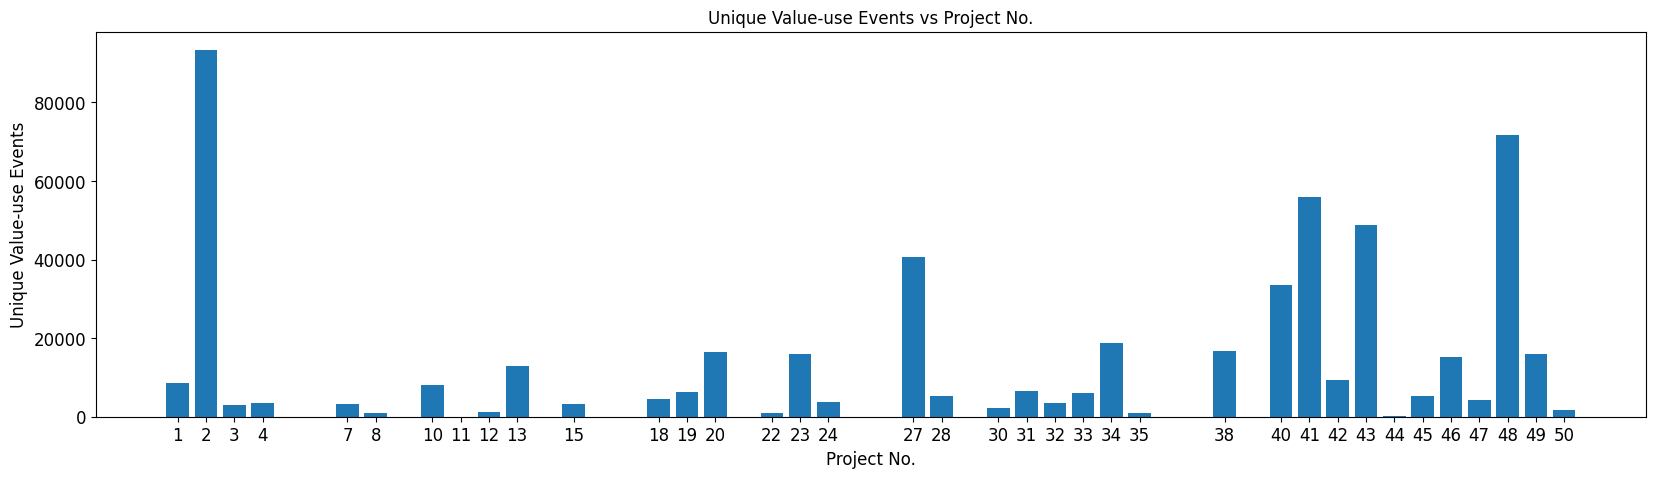
\includegraphics[width=1\linewidth]{figures/evaluation/lex_data_points.png}
    \caption[Unique Value-use Events]{\label{fig:Lex_projects_events}Unique Value-use Events in DyPyBench Projects}
\end{figure}

To evaluate the accuracy of the neural model based on the new data points, we perform a total of 6 experiments using different validation data and the abstraction modes.
Overall, we use 3 different validation data-sets.
First is a random split of 5\% from the data points we found with 37 projects in DyPyBench, second is the data-set provided by the LExecutor. This data-set has data points which were not for training the model.
Finally, the third data-set is the split from the new data points by projects. 6 projects were selected at random, which constitute nearly 5\% of the data points and these projects were excluded from 
training data-set.
For each of the validation data-set we perform 2 experiments, one with the abstraction mode as fine-grained while the other with coarse-grained as described before.

\begin{figure}[ht]
    \centering
    \subfigure[Fine-grained]{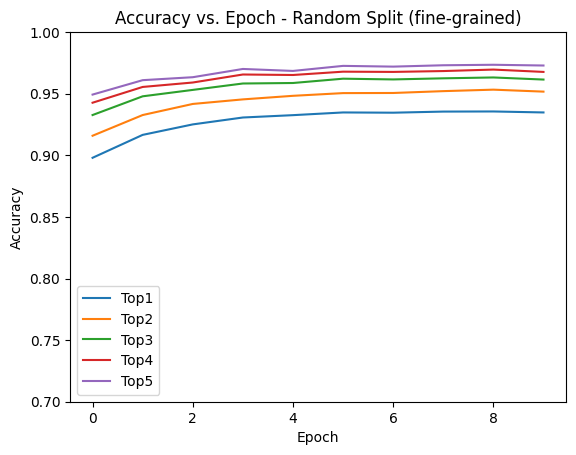
\includegraphics[width=0.4\linewidth]{figures/evaluation/lex_random_fine.png}}
    \subfigure[Coarse-grained]{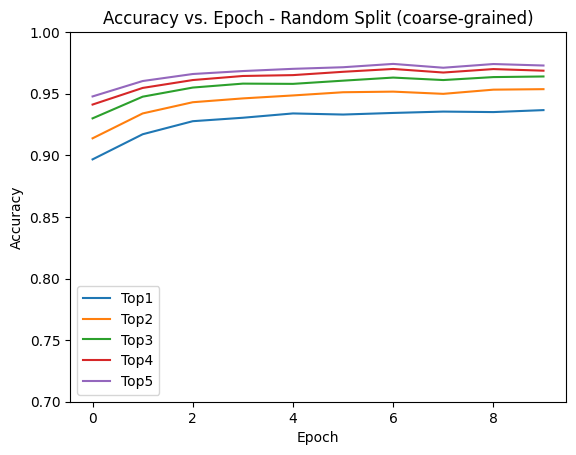
\includegraphics[width=0.4\linewidth]{figures/evaluation/lex_random_coarse.png}}
    \caption[Accuracy vs Epoch (Random Split)]{\label{fig:lex_random}Accuracy vs Epoch (Random Split) }
\end{figure}

Figure \ref{fig:lex_random} shows how the accuracy of the model varies with the number of epochs when the first validation data-set mentioned above is used.
Each line in the Figure \ref{fig:lex_random} shows the accuracy for top-n predictions for the same input.
As can be seen, the accuracy for top-5 is the best followed by top-4 and so on.
We mainly consider the accuracy of the first prediction, which starts at nearly 90\% and improves up to 93\% for both fine and coarse grained.

\begin{figure}[ht]
    \centering
    \subfigure[Fine-grained]{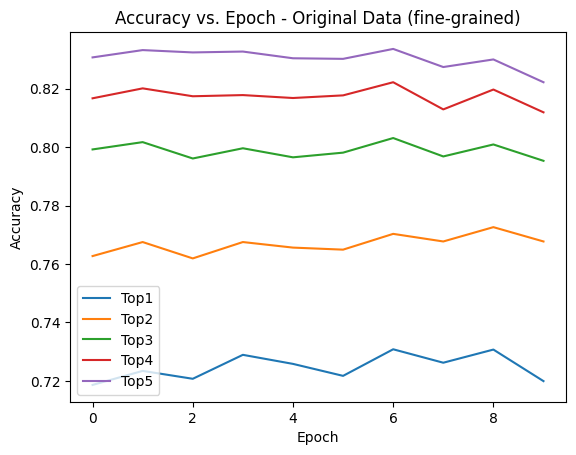
\includegraphics[width=0.4\linewidth]{figures/evaluation/lex_original_fine.png}}
    \subfigure[Coarse-grained]{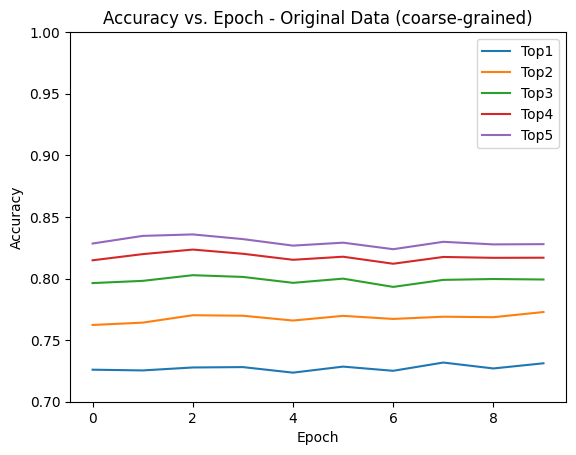
\includegraphics[width=0.4\linewidth]{figures/evaluation/lex_original_coarse.png}}
    \caption[Accuracy vs Epoch (Original Data)]{\label{fig:lex_original}Accuracy vs Epoch (Original Data) }
\end{figure}

Similarly, Figure \ref{fig:lex_original} shows the accuracy versus epoch for validation data-set used by the LExecutor.
As we can see in the Figure \ref{fig:lex_original}, the accuracy is lower than the previous experiments plunging down to 73\% in both cases of abstraction.
Finally, the Figure \ref{fig:lex_project} shows the accuracy versus epoch comparison for the third validation data-set mentioned above.
In this case, the accuracy ranges between the previous two experiments having the value of 85\% for both levels of abstraction.
For the first and second validation data-set, we get the best model in the 7th and 8th epoch.
However, for the third data-set the best model is found at the 4th epoch itself.
Since, the neural model we start with is a pre-trained model, the accuracy range we found is similar to the one specified by LExecutor.

\begin{figure}[ht]
    \centering
    \subfigure[Fine-grained]{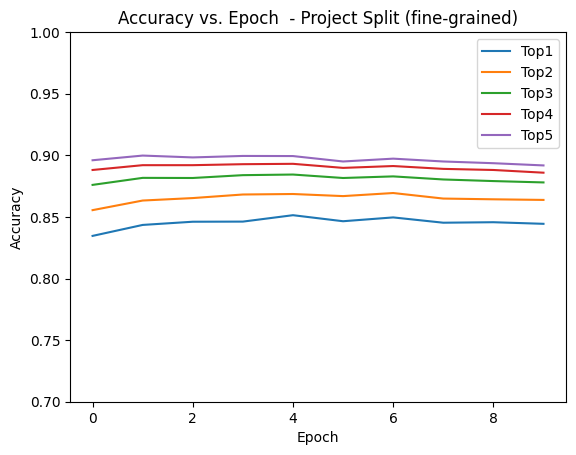
\includegraphics[width=0.4\linewidth]{figures/evaluation/lex_project_fine.png}}
    \subfigure[Coarse-grained]{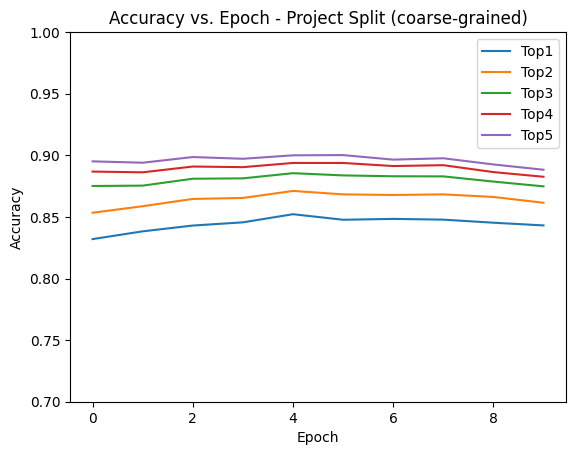
\includegraphics[width=0.4\linewidth]{figures/evaluation/lex_project_coarse.png}}
    \caption[Accuracy vs Epoch (Project Split)]{\label{fig:lex_project}Accuracy vs Epoch (Project Split) }
\end{figure}


\subsection{Effectiveness for Analysis Frameworks}
